\documentclass{article}
\usepackage{amsmath}
\usepackage{fancyhdr}
\usepackage{amsthm}
\usepackage{caption}
\usepackage{amsfonts}
\usepackage{graphicx}
\usepackage{cite}
\usepackage{float}
\theoremstyle{definition}
\newtheorem{theorem}{Theorem}

%\setlength{\intextsep}{0pt}
%\newenvironment{adjustHeight}[1][H]
%  {\captionsetup{abovecaptionskip=-15pt}\begin{listing}[#1]}
%  {\end{listing}}
\linespread{1.3}
\newcommand{\adjustHeight}{\setlength{\abovecaptionskip}{-15pt}} 
\setlength{\belowcaptionskip}{-4pt} 
\newenvironment{sketchproof}{%
  \renewcommand{\proofname}{Sketch of Proof}\proof}{\endproof}
  
\makeatletter
\renewcommand\@biblabel[1]{}
\renewenvironment{thebibliography}[1]
     {\section*{\refname}%
      \@mkboth{\MakeUppercase\refname}{\MakeUppercase\refname}%
      \list{}%
           {\leftmargin0pt
            \@openbib@code
            \usecounter{enumiv}}%
      \sloppy
      \clubpenalty4000
      \@clubpenalty \clubpenalty
      \widowpenalty4000%
      \sfcode`\.\@m}
     {\def\@noitemerr
       {\@latex@warning{Empty `thebibliography' environment}}%
      \endlist}
\makeatother
\setlength{\parindent}{0pt}


\begin{document}


\title{Operational Loss with Correlated Frequency and Severity: an Analytical Approach}
\date{}
\author{Daniel H. Stahl}

\maketitle
Word Count: 3204
\\
\\
Figures and Tables: 9
\\
\\
Acknowledgements: The author reports no conflicts of interest.  The author alone is responsible for the content and writing of the paper.
\newpage
 \begin{abstract}
Operational risk modeling presents a number of difficulties. The severity distribution is often very heavy tailed (moments 2nd order and higher are infinite) making Monte Carlo simulations ineffective.  Analytical solutions like the ``Loss Distribution Approach'' (LDA) model are not flexible enough to model the empirical correlations often found between frequency and severity distributions.  This paper proposes a significant generalization of the LDA model.  This generalization involves treating operational risk as a L\'evy jump-diffusion, which enables auto-correlation in the frequency distribution.  By using a change of measure in the complex domain, this specification also allows for correlation between the severity and frequency distributions. The resulting characteristic function can be numerically approximated by solving a system of differential equations (ODEs).  Using the Runge-Kutta method, the number of steps to retain accuracy throughout the loss distribution is small: in computation tests even 32 steps retained excellent accuracy. This method is tested using three separate severity distributions.  The impact of the resulting correlations on the capital required for operational risk can be large:  in a computational experiment the required capital at the 99.9\% level is over 55\% larger than in a zero-correlation model.  
\\
\\
Core Results:
\begin{enumerate}
\item The model generalizes the LDA framework to include auto-correlation in the frequency distribution and correlation between the frequency and severity distribution.
\item By treating the underlying loss process as a jump-diffusion, the model is dynamic (multi-period).
\item The model retains analytical tractability.
\end{enumerate}

Keywords: L\'evy Process; Correlation; Frequency; Severity; Fourier Inversion; Loss Distribution
\end{abstract}


\newpage
\section{Introduction}

Often the Loss Distribution Approach (LDA) to operational risk assumes that the frequency and severity of operational loss events are independent.  The Basel Committee observes that most banks model frequency and severity separately, with the frequency distribution usually modeled by the Poisson or Negative Binomial distributions (Basel Committee on Banking Supervision, 2011).  This assumption is typically made for computational or estimation purposes.  However, it is not difficult to envisage scenarios where this assumption breaks down in practice.  Following a particularly severe loss event, the manpower required to deal with the event may cause a failure in internal control leading to an increased likelihood of an additional event.  The occurrence of an event may be the result of declining internal controls, which may indicate an increased likelihood of additional events.  In such a scenario the severity of an event impacts the frequency of future events, driving correlation between frequency and severity distributions.  Because of the possibilities of correlation between the frequency and severity of operational loss events, there is no shortage of papers which test the assumption. Several authors (Brechmann et al. 2013, Mittnick et al. 2013) examine the correlation of frequency across business lines.  Cope and Antonini (2008) examine many correlations including correlation between loss event severities.  As a result of the empirical studies around correlation, there has been increased attempts to create models which incorporate correlations.  The Federal Reserve recently released guidance around operational modeling and included a section on diversification modeling (Federal Reserve Board, 2014).  While making no recommendations, the Federal Reserve mentions copula modeling for dependence.  Frachot et al. (2004) attempt to model both correlation between severity and frequency as well as severity auto-correlation, though the model is a single period model which lacks analytic tractability.   B\"ocker and Kl\"uppelberg (2008) propose extensions to the LDA model that uses L\'evy copulas to induce correlation between severity and frequency and has an asymptotically analytic solution.  Peters et al. (2009) propose a model similar to the model in this paper where the frequency and severity distributions are driven by random and correlated factors.  However, their model does not have an analytical solution.
\\
\\
This paper proposes a model that treats the operational risk loss variable as a compound Poisson process. The LDA model is a subset of L\'evy processes which leads to natural extensions including using Carr and Wu's (2004) concept of a ``leverage neutral'' measure.  This method allows for a semi-closed form solution to the distribution of the operational loss random variable while retaining the following key features: the frequency distribution is auto-correlated and the frequency distribution and severity distributions are correlated.  This is achieved by letting the process that describes the frequency distribution jump simultaneously with a severity event.  A severity event hence increases the likelihood of another severity event occurring in any fixed time period following the original event. The standard LDA model is recovered as a special case of this model.

\section{Model Description}
\subsection{Constant Frequency}
Consider a business with operational loss events.  The random variable that counts the number of loss events in a time period \([0, t]\) is \(N_t\) and follows a Poisson distribution with parameter \(\lambda t\).  The total loss from these loss events is \(X_t=\sum_{j=1} ^ {N_t} L_j\) where each \(L_j\) is independently and identically distributed positive random variables with finite expectation.  These \(L_j\) represent the dollar loss from loss event \(j\).  Since each \(L_j\) is stochastic, \(X_t\) is a compound Poisson jump process.  Intuitively, loss events arrive as a ``stream'' instead of at a point in time, with no two events occurring simultaneously.  For notational convenience, \(L_j\) will denote random draws from the relevant distribution while \(L\) will denote the random variable which the relevant distribution describes.  
\\
\\
There is no general analytic formula for the density of a compound Poisson jump process; however the characteristic function has a simple solution.  Recall that the characteristic function of a random variable \(Z\) is defined as \(\mathbb{E}[e^{\mathrm{i}Z}]\) where \(i\) is the number which satisfies \(i^2=-1\).  Hence a compound Poisson process's characteristic function is derived as follows: 
\[\mathbb{E}[e^{u\mathrm{i}X_t}]=\mathbb{E}\left[\mathbb{E}[e^{u\mathrm{i}X_t}|\mathcal{F}_t]\right]=\mathbb{E}\left[\mathbb{E}\left[\prod_{j=1} ^ {N_t} e^{u\mathrm{i} L_j}|\mathcal{F}_t\right]\right]\]
\[=\mathbb{E}\left[\prod_{j=1} ^ {N_t} \mathbb{E}[e^{u\mathrm{i}L}] \right]=\mathbb{E}\left[e^{\mathrm{ln}\left(\mathbb{E}[e^{u\mathrm{i}L}]\right) N_t}\right]\]
\[=e^{\lambda t \left(\mathbb{E}\left[ e^{\mathrm{i}uL}\right]-1\right)}=e^{t \int_{\mathbb{R}} (e^{\mathrm{i}ux}-1) \lambda v(dx)}\]

Where the second line is justified by the moment generating function of a Poisson random variable, \(\mathcal{F}_t\) is the filtration generated by \(N_t\), and \(v\) is the density function of \(L\).  From the characteristic function, it is clear that the jump diffusion is defined by the product \(\lambda v(dx)\) where \(\lambda\) controls the frequency of jumps and \(v(dx)\) controls the jump size. Making this dependence explicit, the characteristic function of a compound Poisson process is denoted
\begin{equation}\phi_P (u;\,\lambda v(dx), t)=e^{t \int_{\mathbb{R}} (e^{\mathrm{i}uL}-1) \lambda v(dx)}\end{equation}
At this point, there is no assumption of correlation between frequency and severity: indeed, the frequency is determined by the constant \(\lambda\).  
\\
\\

L\'evy processes are the set of all continuous processes with independent and stationary increments.  These processes can be specified by their characteristic function, which by the L\'evy-Khintchine representation, is \(e^{t\psi(u)}\) where \(\psi(u)=\mu \mathrm{i} u -\frac{\sigma^2 u^2}{2}+\int_{\mathbb{R}\backslash 0} \left(e^{\mathrm{i} u x}-1-\mathrm{i}ux\mathbb{I}_{|x|<1}\right)dF(x)\). \(\mu\) is the deterministic drift, \(\sigma\) is the diffusion volatility, and \(\int_{\mathbb{R}\backslash 0} \left(e^{\mathrm{i} u x}-1-\mathrm{i}ux\mathbb{I}_{|x|<1}\right)dF(x)\) controls the jump frequency and size.  \(dF(x)\) is a measure which heuristically controls the jumps of \(x\).  Comparing the compound Poisson process to this representation it is clear that \(X_t\) is a L\'evy process (B\"ocker and Kl\"uppelberg 2008).  Cont and Tankov (2004) provides an overview of L\'evy processes in financial modeling while Cruz et al. (2015) and Peters et al. (2015) include the application of L\'evy processes to operational risk modeling.
\subsection{Stochastic Frequency}
The previous section described a process with constant frequency.  In this section this assumption is relaxed.  To create a stochastic frequency, \(t\) itself can be modeled as a random variable.  For notational convenience, when time is modeled as random variable it will be denoted \(\tau\).  In this section \(\tau\) is assumed to be independent of \(L\). 
\\
\\
Time as a random variable is a reasonable model when business events happen with greater or lesser frequency than calendar time.  For example, in times of stress operational decisions tend to be made with increased speed.  The need to make fast and important decisions may decrease clear and dispassionate thought, leading to greater frequency of operational risk events.  Similarly times of relative stability are marked with more deliberation.  
\\
\\
The extended characteristic function for a stochastic and independent \(\tau\) is derived as follows: 
\begin{equation}\label{uncorrelatedCF}\phi_X(u)=\mathbb{E}[e^{u\mathrm{i}X_\tau}]=\theta_\tau \left(\lambda \left(\mathbb{E}\left[e^{\mathrm{i}uL}\right]-1\right)\right)\end{equation}
Where \(\theta_\tau\) is the moment generating function of \(\tau\).  While allowing \(t\) to be stochastic induces stochastic frequency, there still is no assumption of correlation between frequency and severity.
\\
\\
A general specification of \(\tau\) that admits a (semi) analytic moment generating function is the affine jump-diffusion of Duffie et al. (2000). In this paper, \(\tau\) will be driven by a particular form of this general jump-diffusion. However, the independence assumption between \(\tau\) and \(L\) is dropped.  This leads to a model that has increased tail risk to account for dependencies between the frequency and severity distributions.  The goal is to find a semi analytic solution to the characteristic function \(\phi_X(u)\).
\subsubsection{Jump specification}
For this paper, the jump-diffusion that governs \(\tau\) is specified as 
\begin{equation}\tau=\int_0 ^ t v(s)ds\end{equation}
\begin{equation}v_t=v_0+\int_0 ^t a\left(1-\left(\frac{\delta \lambda \mathbb{E}[L]}{a}+1\right)v_s\right)ds+\sigma \int_0 ^ t \sqrt{v_s} dW_s +\delta \sum_{j=1} ^ {N_\tau} L_j \end{equation}
 %Letting \(\bar{k}=\frac{\delta \lambda \mathbb{E}[L]}{a}+1\),
 Letting \(\rho=\delta \lambda \mathbb{E}[L]\),
\begin{equation}\label{tmc}v_t=v_0+\int_0 ^t a\left(1-\left(1+\frac{\rho}{a}\right)v_s\right)ds+\sigma \int_0 ^ t \sqrt{v_s} dW_s +\frac{\rho}{\mathbb{E}[L]\lambda} \sum_{j=1} ^ {N_\tau} L_j \end{equation}
\(N_\tau\) is the time changed counting process \(N_t\).
\\
\\
Modeling \(v_t\) in such a manner has several advantages.  First, by Duffie et al. (2000), \(v_t\) has a semi-analytic moment generating function.  Second, \(v_t\) is positive.  This is necessary as time cannot run backward.  Finally, \(v_t\) is mean reverting.  In the long run \(v_t\) will have an expected value with converges to a one; implying that stochastic time is a long run unbiased estimator of calendar time.  The parameter \(a>0\) controls the speed of reversion to the mean: a higher value indicates a quicker return to ``normal'' levels following an innovation.  The parameter \(\sigma>0\) controls the volatility of the diffusion.  The parameter \(\rho>=0\) controls the impact that a jump has on the diffusion.  A \(\rho\) of \(0\) means that there is no impact (and frequency and severity are uncorrelated).  The ``standard'' LDA model (defined as \(\phi_X(u)=e^{t\lambda \left(\mathbb{E}\left[e^{\mathrm{i}uL}\right]-1\right)}\)) is recovered when \(a=\rho=\sigma=0\).
\subsection{Correlated Frequency and Severity}
This jump-diffusion process for \(v\) provides an auto-correlated frequency of jumps (``clumps'' of jumps) and correlation between the jump size and the frequency of jumps through the jumps' effect on the level of the process \(v\).  Hence this specification fully incorporates correlation between jump size and frequency of jumps and frequency of jumps with itself.  Since there is clear correlation between the jump size and jump frequency, equation \ref{uncorrelatedCF} can no longer be directly applied.  However, Carr and Wu (2004) showed that by using the ``leverage neutral'' measure that the characteristic function of \(X_\tau\) retains analytic tractability under this specification.  
\\
\\
A change of measure occurs as follows: Consider a positive martingale \(Z_t\) which, at the current time \(0\), has a value of one.  Then the expected value of \(Z_t\) is one for for all \(t\).  Now consider the expectation \(\mathbb{E}[Z_t g(Y_t)]\) where \(Y_t\) is another stochastic process.  Then \[\mathbb{E}[Z_t g(Y_t)]=
\int_\Omega Z_t g(Y_t) d\mathbb{P}=
\int_\Omega g(Y_t) \left(Z_t d\mathbb{P}\right)=
\int_\Omega g(Y_t) d\mathbb{\tilde{P}}=\mathbb{\tilde{E}}[g(Y_t)]\] 
Where \(d\mathbb{\tilde{P}}=Z_t d\mathbb{P}\) is a valid density since it satisfies the probability axioms.  In many interesting cases, the change of measure does not fundamentally alter the behavior of the process \(Y_t\); instead simply changing the parameters of the process. 
\\
\\
Changes of measure are frequently used in asset pricing models to switch from the ``physical'' measure to the ``risk-neutral'' measure.  This paper uses the change of measure as a computational trick to induce correlation between the frequency and severity distributions.  For the remainder of this paper frequency and severity are assumed to be correlated.
\subsection{Semi-analytic solution}
The characteristic function of the loss random variable \(X_\tau\) with correlated frequency and severity is 
\[\mathbb{E}[e^{u\mathrm{i}X_\tau}]=\mathbb{E}\left[e^{u\mathrm{i}X_\tau+ \tau \lambda  \left(\mathbb{E}\left[e^{\mathrm{i}uL}\right]-1\right)- \tau \lambda \left(\mathbb{E}\left[e^{\mathrm{i}uL}\right]-1\right)}\right]\]
\[=\mathbb{\hat{E}} \left[e^{\tau \lambda \mathbb{E}\left[e^{\mathrm{i}uL}-1\right]}\right]\]
Where \(\mathbb{\hat{P}}\) is the measure induced by \(\eta_\tau=e^{u\mathrm{i}X_\tau- \tau\lambda \left(\mathbb{E}\left[e^{\mathrm{i}uL}\right]-1\right)}\).  
\begin{theorem}\label{theorem1}
Let \(Y_t\) be a compound Poisson process characterized by \(\lambda v(dx)\).  Define the martingale
\begin{equation}\eta_t=e^{u\mathrm{i}Y_t- t\lambda \left(\mathbb{E}\left[e^{\mathrm{i}uL}\right]-1\right)}\end{equation}
Then under the probability measure \(\hat{d\mathbb{P}}=\eta_t d\mathbb{P}\), \(Y_t\) is a compound Poisson process characterized by \(e^{u\mathrm{i}L}\lambda v(dx)\).
\end{theorem}
\begin{sketchproof}
\[\mathbb{\hat{E}}\left[e^{z\mathrm{i}Y_t}\right]=\mathbb{E}\left[e^{Y_t \mathrm{i} (u+z)-t\lambda \left(\mathbb{E}\left[e^{\mathrm{i}uL}\right]-1\right)}\right]\]
\[=e^{t\lambda \mathbb{E}\left[e^{\mathrm{i}(z+u)L}\right]-t\lambda \mathbb{E}\left[e^{\mathrm{i}uL}\right]}\]
\[=e^{t \int_{R} \left(e^{\mathrm{i}zx}-1\right)\lambda e^{\mathrm{i}uL}v(dx)}=\phi_{P} (z;\,e^{u\mathrm{i}x}\lambda v(dx), t)\]
\end{sketchproof}

Carr and Wu (2004) prove that this theorem remains applicable with \(\tau\) substituted for \(t\).  This theorem implies that under this new measure, the dynamics of \(v\) are as follows:
\begin{equation}\label{tmcLN}v_t=v_0+\int_0 ^t a\left(1-\left(\frac{\rho}{a}+1\right)v_s\right)ds+\sigma \int_0 ^ t \sqrt{v_s} dW_s +\frac{\rho}{\mathbb{E}[L] \lambda} \sum_{j=1} ^ {\hat{N}_\tau} L_j \end{equation}
Where \(\hat{N}_\tau\) is the time-changed counting process under the ``leverage-neutral'' measure.   By Duffie et al. (2000) and theorem \ref{theorem1}, for the affine process \(v_t\), the following statement holds:
\[\mathbb{E} \left[e^{-r\int_0 ^ {T} v_s ds}\right]=e^{\gamma(0, T)+\zeta(0, T)v_0}\]
Where \(\gamma,\,\zeta\) satisfy
\[
\begin{cases}
\frac{\partial \zeta}{\partial t}=a\left(1+\frac{\rho}{a}\right) \zeta+r-\frac{1}{2} \sigma^2 \zeta^2 - \int_{\mathbb{R}} \left(e^{\frac{\rho \zeta x}{\mathbb{E}[L] \lambda}}-1\right)\lambda e^{u\mathrm{i}x} v(dx) & \zeta(T, T)=0\\
\frac{\partial \gamma}{\partial t}=-a \zeta & \gamma(T, T)=0
\end{cases} \]

Note that \(\int_{\mathbb{R}} \left(e^{\frac{\rho \zeta x}{\mathbb{E}[L] \lambda}}-1\right)\lambda e^{u\mathrm{i}x} v(dx) = \lambda \mathbb{E}\left[ e^{ \frac{\rho \zeta L }{\mathbb{E}[L] \lambda}+u\mathrm{i} L}\right] - \lambda \mathbb{E}\left[ e^{u\mathrm{i} L} \right] \).  Since the time-changed characteristic function is \(\mathbb{\hat{E}}\left[e^{\psi(u)\tau} \right] \),  \(r=-\psi(u)=\lambda(1-\mathbb{E}[e^{u\mathrm{i}L}])\).  Making these subsitutions, the system of ODEs becomes

\begin{equation}\label{ode}
\begin{cases}
\frac{\partial \zeta}{\partial t}=(a+\rho) \zeta-\lambda\left(\phi_L(u-\mathrm{i}\frac{\rho}{\mathbb{E}[L] \lambda} \zeta )-1\right)-\frac{1}{2} \sigma^2 \zeta^2 & \zeta(T, T)=0\\
\frac{\partial \gamma}{\partial t}=-a \zeta & \gamma(T, T)=0
\end{cases} \end{equation}
Where \(\phi_L(z)\) is the characteristic function of \(L\).

\section{Severity Distribution}
Mathematically, any distribution with analytic characteristic function can be used as a severity distribution.  Due to the nature of loss events this distribution must have support constrained to the positive reals. This paper examines three severity distributions to demonstrate the capabilities of the model.

\subsection{Gamma Distribution}

The Gamma distribution is a two parameter distribution with the following features (Johnson et al. 1994):

\begin{center}
\begin{tabular}{lc}
Density: & \(\frac{1}{\Gamma(\alpha)\alpha^\beta}x^{\alpha-1} e^{-\frac{x}{\beta}}\)\\
Expectation: & \(\alpha \beta\) \\
Variance: & \(\alpha \beta^2\) \\
Characteristic function: & \((1-\beta u\mathrm{i})^{-\alpha} \)
\end{tabular}
\end{center}


This distribution's simple density, moments, and characteristic function makes for convenient analytical analysis and behaves well numerically.  To avoid confusion, the parameters for the Gamma distribution will be denoted as follows: \(\alpha_G\), \(\beta_G\).

\subsection{Inverse Gaussian Distribution}

The Inverse Gaussian distribution results from letting the standard deviation of the Gaussian density be used as a random variable.  The distribution is parameterized by \(\mu_{IG}\) and \(\lambda_{IG}\) and has the following features (Johnson et al. 1994):


\begin{center}
\begin{tabular}{lc}
Density: & \(\sqrt{\frac{\lambda_{IG}}{2\pi x^3}}e^{\frac{-\lambda(x-\mu)^2}{2\mu^2 x}}\)\\
Expectation: & \(\mu\) \\
Variance: & \(\frac{\mu^3}{\lambda_{IG}}\) \\
Characteristic function: & \(e^{\frac{\lambda_{IG}}{\mu} \left(1-\sqrt{1-\frac{2\mu^2 u\mathrm{i}}{\lambda_{IG}}}\right)}\)
\end{tabular}
\end{center}

Like the Gamma distribution, the Inverse Gaussian distribution has simple density, finite moments (if \(\lambda_{IG}>0\)), and an analytic characteristic function.

\subsection{Stable Distribution}

There is a substantial body of literature (Rachev et al. 2006, Gourier et al. 2009, Kerbl 2014) providing empirical evidence for ``fat-tailed'' (infinite variance) severity distributions. The stable distribution is a four parameter distribution with the following features (Voit 2003):\footnote{The characteristic function is valid for \(u>0\) and \(\alpha>1\)}

\begin{center}
\begin{tabular}{lc}
Density: & No closed form density (in general)\\
Expectation: & \(\mu\) when \(\alpha \in (1,\,2]\)\\
Variance: & Infinite (in general)\\
Characteristic function: & \(e^{iu\mu-(cu)^\alpha \left(1-\beta \mathrm{i} \tan\left(\frac{\pi \alpha}{2}\right)\right)}\)
\end{tabular}
\end{center}


In general, the stable distribution has support on the reals.  When \(\beta=1\) the distribution decays quickly to the left while the right tail remains ``fat''.  The probability of a negative outcome can be made infinitesimal by an appropriate choice of \(\mu\) and \(c\).  To retain finite expectation (a requirement for \(\hat{b}\) to be positive) \(\alpha\) is constrained to within \((1,\, 2]\).  The shift parameter \(\mu\) and the scale parameter \(c\) are free parameters which can be calibrated to the historical data.  


This distribution was leveraged by Carr and Wu (2003) to model asset returns: with \(\beta=\pm 1\) (maximum skewness) the infinite variance results from thick tails in only one direction. Hence option pricing (which requires finite variance of the asset) and severity modeling (which requires positive severities) can be safely modeled with the stable distribution with maximum skewness.   
\\
\\
The infinite variance of this class of distribution makes many numerical solutions, such as Monte Carlo methods, slow to converge (Brunner et al. 2009).  By using the numerical method described below these numerical issues are circumvented. To avoid confusion, the parameters for the Stable distribution will be denoted as follows: \(\alpha_S\), \(\beta_S\),  \(\mu_{S}\), \(c_{S}\).

\section{Numerical Implementation}
\subsection{Severity Distributions}
To test the numerical inversion of the distributions, the following severity distributions were chosen:
\begin{enumerate}
\item Gamma\((6.5, 200)\)
\item Inverse Gaussian\((1300, 5000)\)
\item Stable\((1.1, 1, 1300, 100)\)
\end{enumerate}
These parameters were chosen to have expectation of \(1300\). The plots of these distributions are as follows:
\begin{figure}[H]
\adjustHeight

\centering
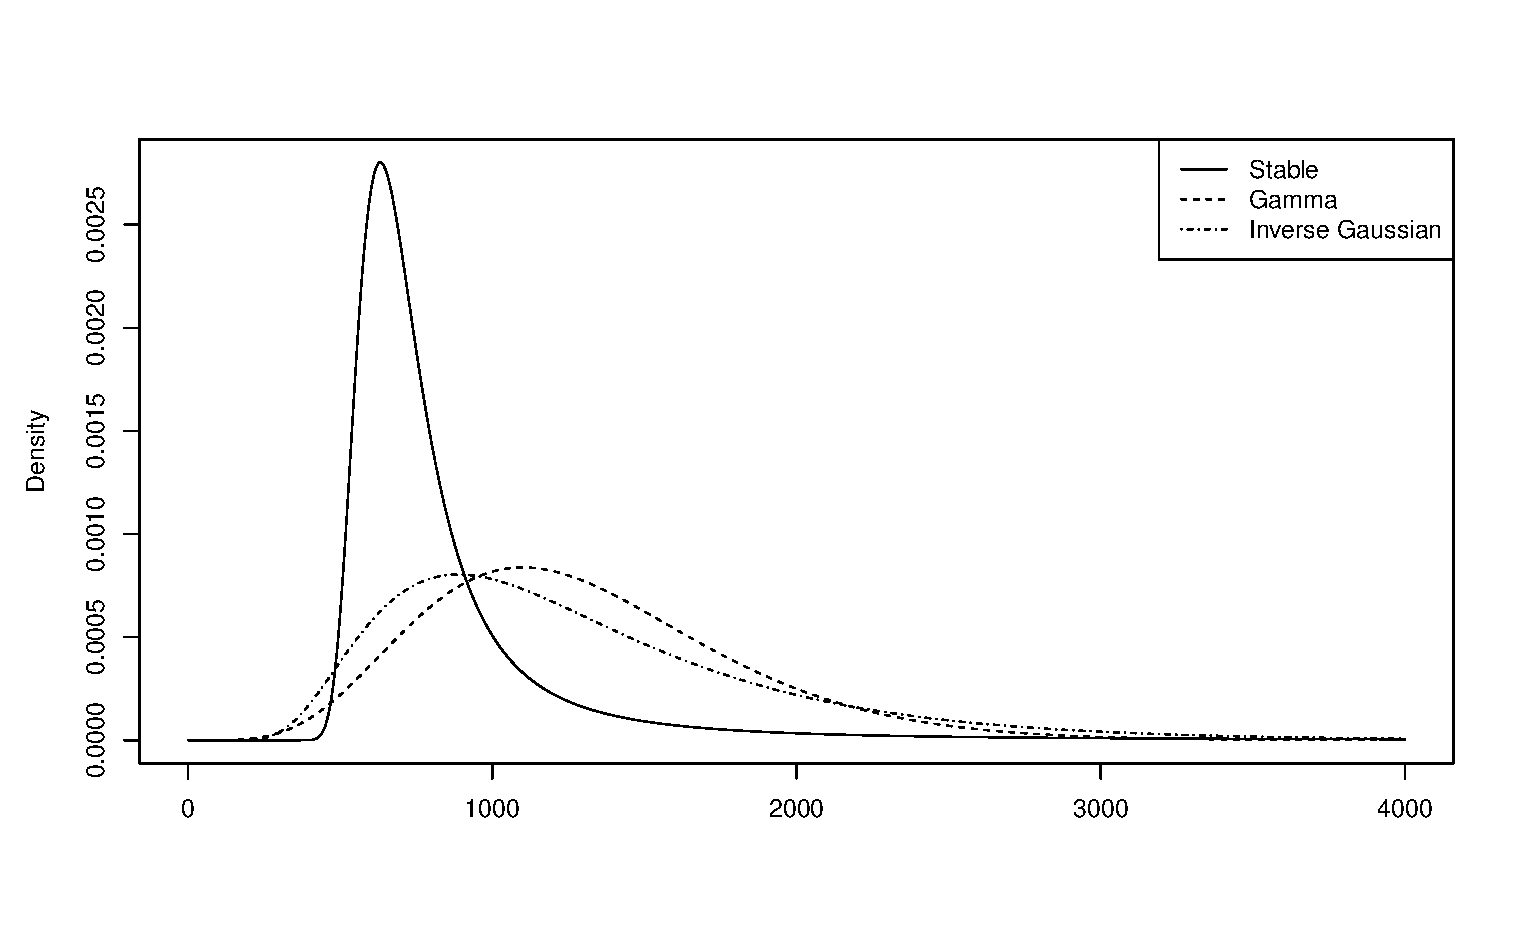
\includegraphics[width=1\textwidth]{Figure1}
\caption{\(\alpha_G=6.5\), \(\beta_G=200\), \(\mu_{IG}=1300\), \(\lambda_{IG}=5000\), \(\alpha_{S}=1.1\), \(\beta_{S}=1\), \(c_{S}=100\), \(\mu_{S}=1300\)}
\end{figure}

Note that the Gamma and Inverse Gaussian distributions are much wider over much of the domain; this is due to the rapidity that the tails approach zero relative to the Stable distribution.
\subsection{Solving the Differential Equations}
The equations (\ref{ode}) can be numerically solved using the Runge-Kutta method. This method features fourth order convergence (Press et al. 1992) resulting in highly accurate results for even fairly large step sizes.  The accuracy of the results will be explored in a later section. The Runge-Kutta, like all numerical solutions to ODEs, discretizes the domain of the function.  The Runge-Kutta uses finite-difference approximations to the derivative of the function in order to compute the solution.  The Runge-Kutta improves over naive solutions like Euler's method by taking the ``average'' of several function solutions in the area of the discrete step.  The scheme is given explicitly as follows:
\[
\left[\begin{array}{c}
\zeta_{j+1} \\
\gamma_{j+1}
\end{array}\right] =
 \left[\begin{array}{c}
\zeta_{j}\\
\gamma_j
\end{array} \right]
+\frac{1}{6}k_1+\frac{1}{3} k_2+\frac{1}{3} k_3+\frac{1}{6} k_4
\]
Where the \(k_i\) are defined as follows:
\[\def\arraystretch{1.8}\begin{array}{l} 
k_1=h \left[\begin{array}{c} f(jh, \gamma_j, \zeta_j) \\ g(jh, \gamma_j, \zeta_j) \end{array} \right] \\
k_2= h \left[\begin{array}{c} f\left(\left(j+\frac{1}{2}\right)h, \gamma_j+\frac{1}{2}k_1, \zeta_j + \frac{1}{2} k_1\right) \\ g\left(\left(j+\frac{1}{2}\right)h, \gamma_j+\frac{1}{2}k_1, \zeta_j + \frac{1}{2} k_1\right) \end{array} \right]\\
k_3= h \left[\begin{array}{c} f\left(\left(j+\frac{1}{2}\right)h, \gamma_j+\frac{1}{2}k_2, \zeta_j + \frac{1}{2} k_2\right) \\ g\left(\left(j+\frac{1}{2}\right)h, \gamma_j+\frac{1}{2}k_2, \zeta_j + \frac{1}{2} k_2\right) \end{array}\right]\\
k_4= h \left[\begin{array}{c} f\left(\left(j+1\right)h, \gamma_j+k_3, \zeta_j +  k_3\right) \\ g\left(\left(j+1\right)h, \gamma_j+k_3, \zeta_j +  k_3\right) \end{array} \right]
\end{array}
\]
Here \(h=\frac{t}{n}\) where \(n\) is the number of steps in the algorithm, \(j\) is the \(j\)'th step, and \(f\) and \(g\) are the following functions:
\[f(t, \gamma, \zeta)=\lambda\phi_L(-(u+\delta \zeta)\mathrm{i})+\frac{1}{2} \sigma^2 \zeta^2 -a(\bar{k}+1) \zeta-\lambda\]
\[g(t, \gamma, \zeta)=a\zeta\]

\subsection{Analysis of Complexity}
The complexity for computing the characteristic function for a given \(u\) is \(O(n)\) where \(n\) is the number of discrete steps in the Runge-Kutta method.  To numerically invert the characteristic function, \(u\) must be discretized as well.  Hence to compute an array of approximate \(\phi_X\) requires \(O(nm)\) where \(m\) is the number of discrete steps in the complex domain.  
\\
\\
Inverting the characteristic function to recover the density using the method proposed by Fang and Oosterlee (2008) requires \(O(mq)\) operations where \(q\) is the number of steps in real domain.  The total complexity is thus \(O(m(n+q))\).  
\\
\\
Fixing \(q\) at \(1024\) and \(m\) at \(256\), the speed using C++ and 4 threads of a fifth generation Intel Core i5-5250U is the following for each \(n\):

\begin{center}
\begin{tabular}{c|c|c|c}
& \(n=128\) & \(n=32\) & \(n=2\)\\
\hline
Milliseconds & \(50\) & \(23\) & \(15\)
\end{tabular}
\end{center}

Even with \(n=128\) the time it takes to run the algorithm is barely perceptible to humans; while with \(n=2\) the result appears instant to the human perception. The speed of the algorithm does not show linear improvement in \(n\) since the \(mq\) operations from the inversion algorithm remains fixed as \(n\) varies. The algorithm proposed by Fang and Oosterlee is embarrassingly parallel and using multiple cores is trivial using, for example, Open-MP.

\subsection{Analysis of Accuracy}

The accuracy of Fang and Oosterlee's algorithm is well documented in their paper.  The accuracy of the Runge-Kutta algorithm is thus investigated in this paper.  The following plots show the accuracy of the density for various \(n\) for the Stable severity distribution.

\begin{figure}[H]
Absolute difference between densities with \(\alpha_S=1.1\), \(\beta_S=1\), \(c_S=100\), \(\mu_S=1300\), \(\lambda_S=100\),  \(t=1\), X steps\(=1024\), U steps\(=256\), \(a=.4\), \(\sigma=.4\), \(\delta=6.923077e-06\) 

\centering
\begin{minipage}{0.48\textwidth}
\centering
\includegraphics[width=1\textwidth]{Figure2}
\caption{\(n=128\) vs \(n=32\)}
\end{minipage}\hfill
\begin{minipage}{0.48\textwidth}
\centering
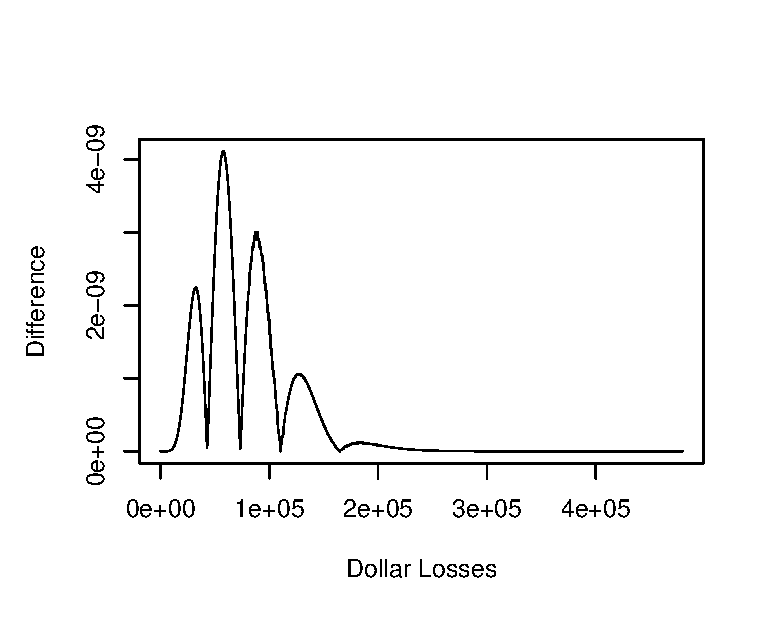
\includegraphics[width=1\textwidth]{Figure3}
\caption{\(n=128\) vs \(n=2\)}
\end{minipage}
\end{figure}

The difference between the accuracy using \(n=128\) and \(n=32\) is exceedingly small.  What is perhaps most surprising is that even with \(n=2\) the accuracy is still acceptable especially in the tails.  

\subsection{Plot of Results}

The following plots and tables show the output from this model using a reasonable parameterization for the three chosen severity distributions.  Figures (\ref{comparePlotsGamma}), (\ref{comparePlotsIG}), and (\ref{comparePlotsStable}) compare the results from the ``standard'' LDA and the extension proposed in this paper.  Even without correlation between the severity and frequency distribution there is substantially more variation resulting from the auto-correlation of the frequency distribution. As expected, the ``fattest'' tail results from the distribution with the largest \(\delta\). The distributions with Gamma and Inverse Gaussian severities are very similar shaped as expected for distributions with ``thin'' tails. Since the expected values of the distributions remain similar as the correlation becomes greater the distributions shift.  Small values and large values become more likely.   

\begin{figure}[H] 
\adjustHeight

\centering
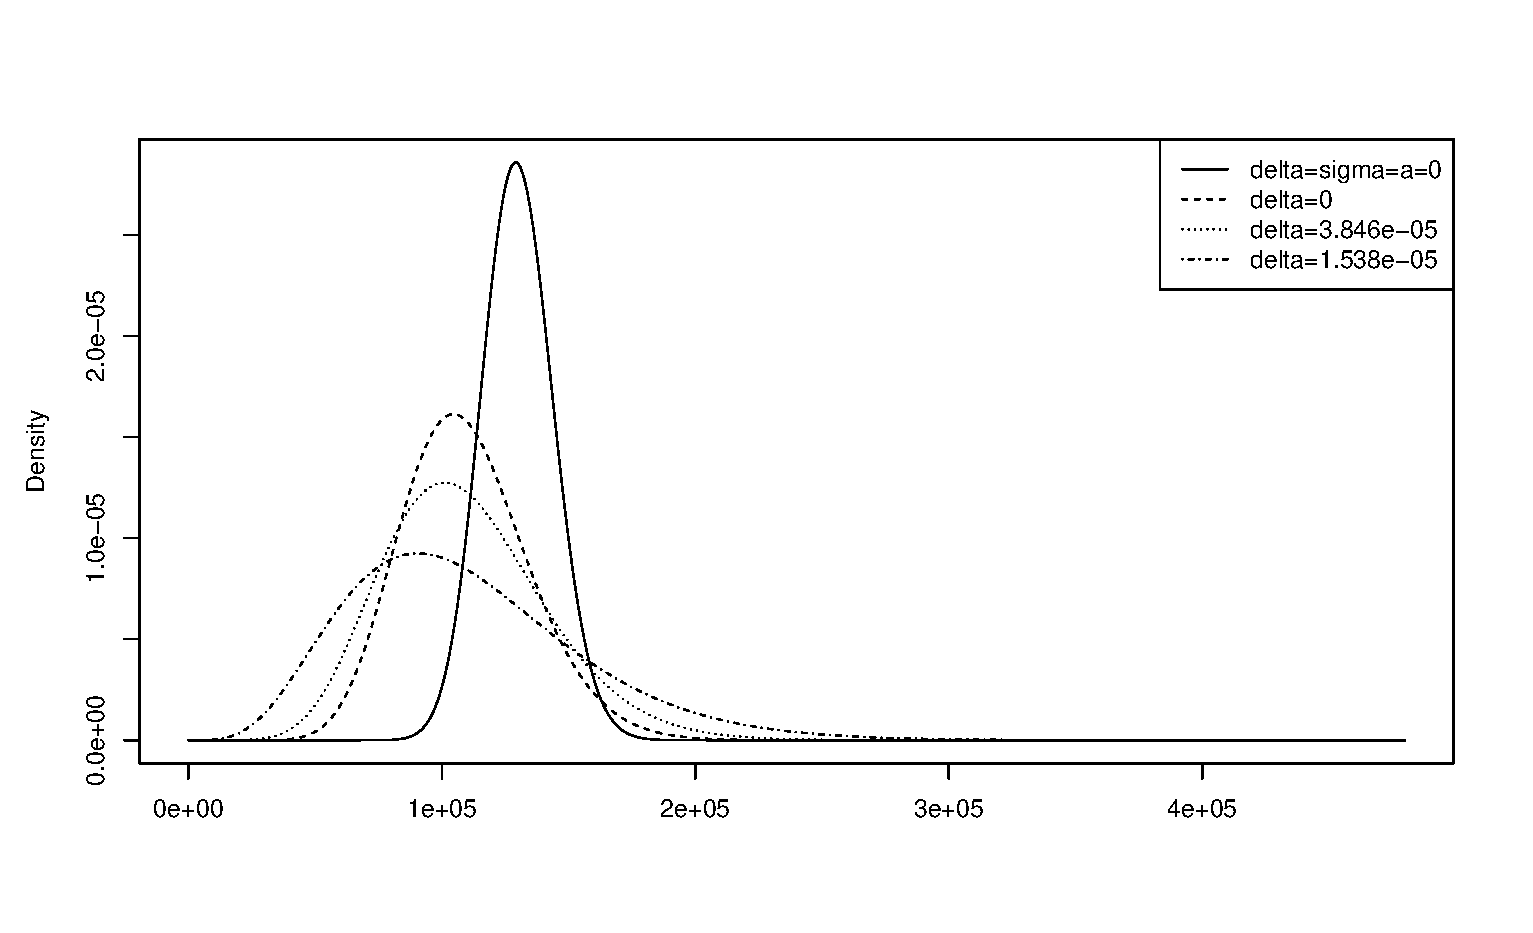
\includegraphics[width=1\textwidth]{Figure4}
\caption{Gamma Severity: \(\alpha_G=6.5\), \(\beta_G=200\), \(\lambda=100\),  \(t=1\), ODE steps\(=128\), X steps\(=1024\), U steps\(=256\)}\label{comparePlotsGamma}
\end{figure}

\begin{figure}[H] 
\adjustHeight

\centering
\includegraphics[width=1\textwidth]{Figure5}
\caption{Inverse Gaussian Severity: \(\mu_{IG}=1300\), \(\lambda_{IG}=5000\), \(\lambda=100\),  \(t=1\), ODE steps\(=128\), X steps\(=1024\), U steps\(=256\)}\label{comparePlotsIG}
\end{figure}

\begin{figure}[H] 
\adjustHeight

\centering
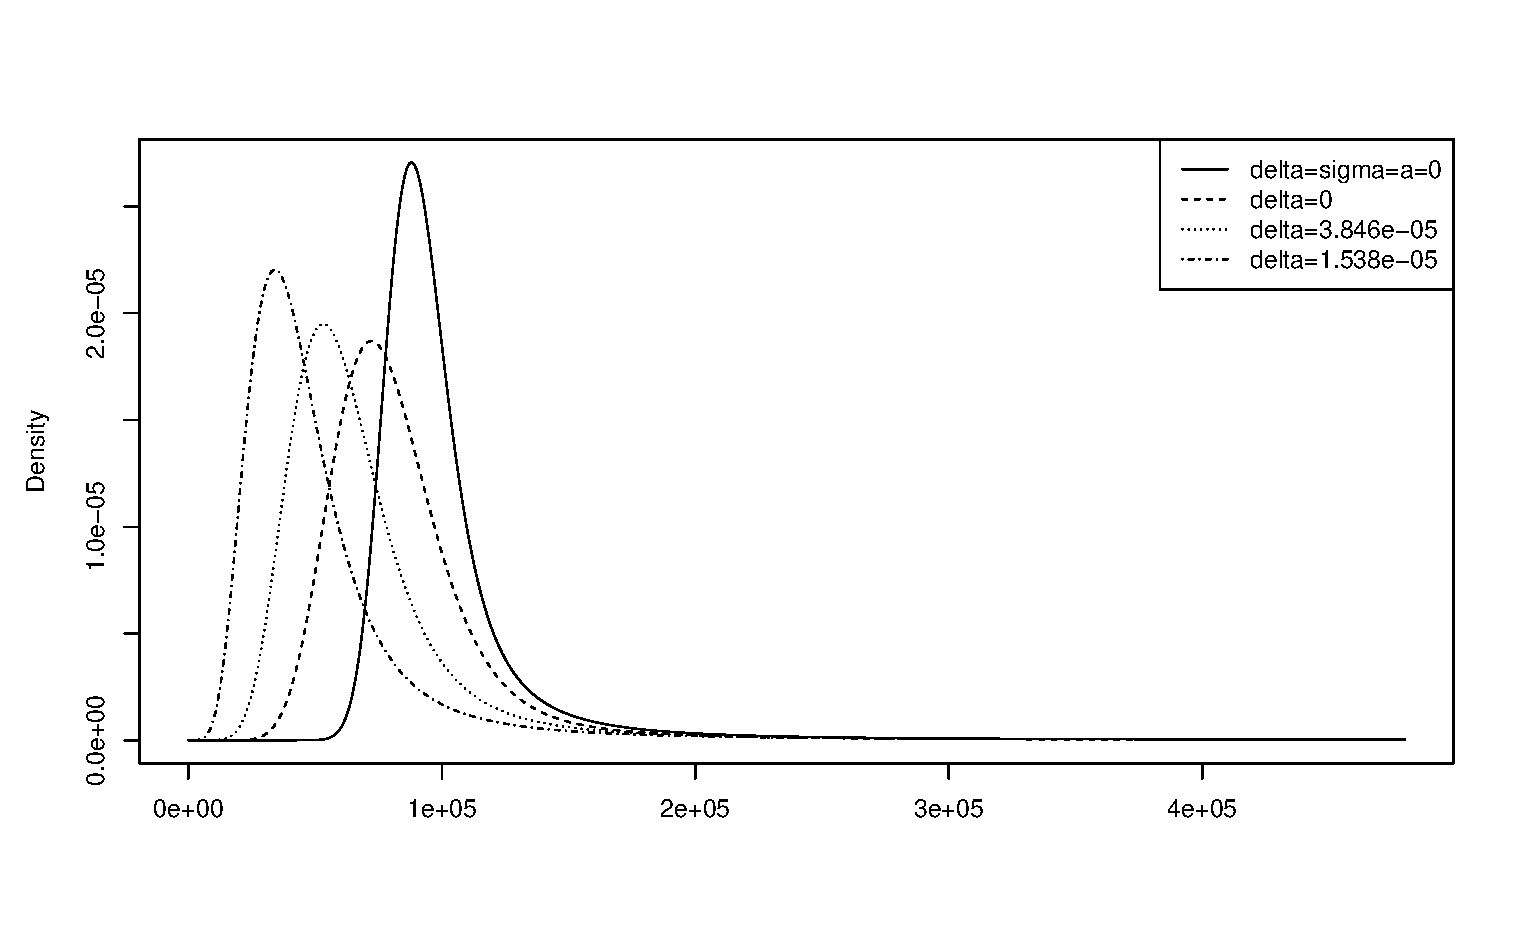
\includegraphics[width=1\textwidth]{Figure6}
\caption{Stable Severity: \(\alpha_S=1.1\), \(\beta_S=1\), \(c_S=100\), \(\mu_S=1300\), \(\lambda=100\),  \(t=1\), ODE steps\(=128\), X steps\(=1024\), U steps\(=256\)}\label{comparePlotsStable}
\end{figure}

Most firms use a value at risk measure to allocate capital.  The parameter \(\delta\) has a large impact on the \(99.9\%\) value at risk for every severity distribution:

\begin{center}
\begin{tabular}{c|c|c|c}
\(\delta\) & \(0\) & \(3.846e-05\) & \(1.538e-05\)\\
\hline
VaR & \(201,760\) & \(233,196\) & \(305,924\) \\
Increase over \(\delta=0\) & 0\% & 15.58\% & 51.63\%
\end{tabular}
\end{center}
\captionof{table}{Gamma Severity: \(\alpha_G=6.5\), \(\beta_G=200\), \(\lambda=100\),  \(t=1\), \(a=\sigma=.4\)} \label{table1}
\vspace{10mm}
\begin{center}
\begin{tabular}{c|c|c|c}
\(\delta\) & \(0\) & \(3.846e-05\) & \(1.538e-05\)\\
\hline
VaR & \(203,167\) & \(236,950\) & \(315,777\)\\
Increase over \(\delta=0\) & 0\% & 16.63\% & 55.43\%
\end{tabular}
\end{center}
\captionof{table}{Inverse Gaussian Severity: \(\mu_{IG}=1300\), \(\lambda_{IG}=500\), \(\lambda=100\),  \(t=1\), \(a=\sigma=.4\)} \label{table2}
\vspace{10mm}
\begin{center}
\begin{tabular}{c|c|c|c}
\(\delta\) & \(0\) & \(3.846e-05\) & \(1.538e-05\)\\
\hline
VaR & \(1,824,450\) & \(2,390,830\) & \(2,608,860\)\\
Increase over \(\delta=0\) & 0\% & 31.04\% & 43.00\%
\end{tabular}
\end{center}
\captionof{table}{Stable Severity: \(\alpha_S=1.1\), \(\beta_S=1\), \(c_S=100\), \(\mu_S=1300\), \(\lambda=100\),  \(t=1\), \(a=\sigma=.4\)} \label{table3}
\vspace{10mm}

Again, the Gamma and Inverse Gaussian severities are remarkably similar while the Stable distribution has VaR over an order of magnitude larger.  The correlation parameter also has more impact on the Stable severity than for the other distributions.

\section{Estimation}

For estimation purposes, it is assumed that operational loss data is provided which has the dollar severity and time-stamp for each loss event.  The severity distribution may be estimated using standard maximum likelihood methods from the severity field in the data.  The frequency process is somewhat more involved since the latent process \(v_t\) is unobserved.  There are five parameters that must be estimated: \(v_0\), \(\delta\), \(a\), \(\sigma\), and \(\lambda\).  To estimate these parameters, the operational loss data must be partitioned into segregated time intervals.  These partitions should be large enough that loss data exists in each partition, but small enough to provide an appropriately rich data set.  Once this data set is obtained, the maximum likelihood technique of Singleton (2001) can be used.  This technique involves finding the conditional characteristic function and inverting it for each loss value obtained from the partitioned data.  While this appears at first glance to be inefficient, the algorithm used to invert the characteristic function need only be run once for each iteration of the maximum likelihood algorithm.  Hence a single pass through the partitioned data has similar complexity as inverting the distribution.  The log-likelihood function of the parameter vector \(\omega\) is 
\[\mathcal{L}(\omega)=\sum_{j} \mathrm{log}\left((\hat{f}\left(\omega; x_{t_j}\right)\right)\]
Where \(j\) iterates over the partitioned data and \(x_{t_j}\) is the dollar loss in partition \(j\).
\section{Conclusion}

The model presented in this paper provides a method new to the operational risk literature for correlating between severity and frequency in an LDA framework.  This model substantially extends the traditional LDA modeling approach by allowing the model to be time-dependent, with stochastic and mean-reverting frequency.  The frequency jumps simultaneously with the severity events; inducing correlation between frequency and severity. The flexibility of the model allows firms to more precisely estimate the capital to hold for operational risk and design superior controls to mitigate operational risk.  Since the LDA model is a nested model, firms can also test whether the LDA modeling approach is robust to correlations between frequency and severity and auto-correlations between frequency.
\\
\\
While the model substantially generalizes the standard LDA model, there is still room for additional extensions.  For example, the Basel committee requires \(56\) separate operational loss ``bins'': seven risk types across eight business lines (Basel Committee on Banking Supervision, 2006).  These risk and business types can be modeled by a multidimensional frequency distribution.  In this way the severities across risk and business type will be independent, but a severe event in one business line or risk will directly impact the frequency of severe events in every other risk or business line. 

\newpage
\begin{thebibliography}{9}
\bibitem{basel2006}
Basel Committee on Banking Supervision. International Convergence of Capital
Measurement and Capital Standards: A Revised Framework. Technical report, Bank for International Settlements, 2006.
\bibitem{basel2011}
Basel Committee on Banking Supervision. Operational Risk - Supervisory Guidelines for the Advanced Measurement Approaches. Technical report, Bank for International Settlements, 2011.
\bibitem{BCC141}
BCC 14-1.  Supervisory Guidance for Data, Modeling, and Model Risk Management under the Operational Risk Advanced Measurement Approaches.  Technical report, Federal Reserve Board, 2014.
\bibitem{Bocker2008}
K. B\"ocker, C. Kl\"uppelberg.  Modeling and Measuring Multivariate Operational Risk with L\'evy Copulas.  \textit{Journal of Operational Risk}, 3, 2008.
\bibitem{Brechmann2013}
E. C. Brechmann, C. Cxado, and S. Paterlini.  Flexible Dependence Modeling of Operational Risk Losses and Its Impact on Total Capital requirements.  \textit{Journal of Banking and Finance}, 40, 2014.
\bibitem{Brunner2009}
M. Brunner, F. Piacenza, F. Monti, and D. Bazzarello.  Fat Tails, Expected Shortfall and the Monte Carlo Method: a Note.  \textit{Journal of Operational Risk}, 4, 2009.
\bibitem{Carr2003}
P. Carr and L. Wu.  The Finite Moment Log Stable Process and Option Pricing.  \textit{Journal of Finance}, 58, 2003.
\bibitem{Carr2004}
P. Carr and L. Wu. Time-changed L\'evy Processes and Option Pricing.  \textit{Journal of Financial Economics}, 71, 2004.
\bibitem{Cont2004}
R. Cont and P. Tankov. \textit{Financial Modelling with Jump Processes}. Chapman \& Hall/CRC, London, UK, 2004.
\bibitem{Cope2008}
E. Cope and G. Antonini.  Observed Correlations and Dependencies Among Operational Losses in the ORX Consortium Database.  \textit{Journal of Operational Risk}, 3, 2008.
\bibitem{Cruz2015}
M. Cruz, G. Peters, P. Shevchenko. \textit{Fundamental Aspects of Operational Risk and Insurance Analytics}. John Wiley \& Sons, New York, USA, 2015.
\bibitem{Duffie2000}
D. Duffie, J. Pan, and K. Singleton.  Transform Analysis and Asset Pricing for Affine Jump-diffusions.  \textit{Econometrica}, 68, 2000.
\bibitem{Fang2008}
F. Fang and C. W. Oosterlee.  A Novel Pricing Method of European Options based on Fourier-cosine Series Expansions.  \textit{SIAM Journal of Scientific Computing}, 31, 2008.
\bibitem{Frachot2004}
A. Frachot, T. Roncalli, and E. Salomon.  The Correlation Problem in Operational Risk. \textit{Credit Agricole}, 2004.
\bibitem{Gourier2009}
E. Gourier, W. Farkas, and D. Abbate.  Operational Risk Quantification using Extreme Value Theory and Copulas: from Theory to Practice.  \textit{Journal of Operational Risk}, 4, 2009
\bibitem{Johnson1994}
N. Johnson, S. Kotz, N. Balakrishnan.  \textit{Continuous Univariate Distributions}.  John Wiley \& Sons, New York, USA, 1994.
\bibitem{Kerbl2014}
S. Kerbl.  Evidence, Estimates, and Extreme Values from Austria.  \textit{Journal of Operational Risk}, 9, 2014.
\bibitem{Mittnik2013}
S. Mittnik, S. Paterlini, and T. Yener.  Modeling Dependence of Operational Loss Frequencies.  \textit{Journal of Operational Risk}, 8, 2013.
\bibitem{Peters2009}
G. Peters, P. Shevchenko, M. W\"uthrich.  Dynamic Operational Risk: Modeling Dependence and Combining Different Sources of Information.  \textit{Journal of Operational Risk}, 4, 2009.
\bibitem{Peters2015}
G. Peters and P. Shevchenko.  \textit{Advances in Heavy Tailed Risk Modeling: A Handbook of Operational Risk}. John Wiley \& Sons, New York, USA, 2015.
\bibitem{Press1992}
W. Press, B. Flannery, S. Teukolsky, and W. Vetterling.  \textit{Numerical Recipes in FORTRAN 77: The Art of Scientific Computing}.  Cambridge University Press, Cambridge, England, 2nd Edition, 1992.
\bibitem{Rachev2006}
S. Rachev, A. Chernobai, and C. Menn.  Empirical Examination of Operational Loss Distributions.  M. Morlock, C. Schwindt, N. Trautmann, and J. Zimmermann, editors, \textit{Perspectives on Operations Research}, pages 379-401.  Deutscher Universit\"{a}ts-Verlag/GWV Fachverlage GmbH, Wiesbaden, 2006.
\bibitem{Singleton2001}
K. Singleton.  Estimation of Affine Asset Pricing Models using the Empirical Characteristic Function.   \textit{Journal of Econometrics}, 102, 2001.
\bibitem{Voit2003}
J. Voit. \textit{The Statistical Mechanics of Financial Markets}. Springer-Verlag, 2nd Edition, 2003.
\end{thebibliography}


\end{document}
